% Make to Innovate Milestone Template
% Modified from the UCT Project report by Linus C. Brendel
% https://www.overleaf.com/latex/templates/uct-report-template/grctkzjtrqrm

%------------------------------------------------------
% DO NOT MODIFY THE FOLLOWING
\documentclass[12pt]{article}
\usepackage[english]{babel}
\usepackage{natbib}
\bibliographystyle{chicago}
\usepackage{url}
\usepackage{listings}
\usepackage{color} %red, green, blue, yellow, cyan, magenta, black, white
\usepackage[utf8x]{inputenc}
\usepackage{amsmath}
\usepackage{amsthm}
\usepackage{mathtools}
\usepackage{lmodern}
\usepackage{multirow}
\usepackage{pgfplots}
\theoremstyle{definition}
\newtheorem{definition}{Definition}[section]
%\theoremstyle{etape}
%\newtheorem{etape}{Etape}[section]
\theoremstyle{definition}
\newtheorem{etape}{Etape}
\newtheorem*{remark}{Remark}
\usepackage{graphicx}
\usepackage[numbered,framed]{matlab-prettifier}
\usepackage{filecontents}
\usepackage{mdframed}
\usepackage{xcolor}
\usepackage{etoolbox}

% define a style
\mdfdefinestyle{mathbackground}{
    hidealllines=true,
    backgroundcolor=black!20,
    skipbelow=\baselineskip,
    skipabove=\baselineskip,
    innertopmargin=1pt,
}

% add it to {equation}
\surroundwithmdframed[style=mathbackground]{eqnarray}
% ... similar for other environments

% add the environment to \[\] (needs etoolbox)
\preto{\[}{%
    \begin{mdframed}[style=mathbackground]%
    \vspace{-\baselineskip}%
}
\appto{\]}{%
    \end{mdframed}%
}

\graphicspath{{images/}}
\usepackage{parskip}
\usepackage{fancyhdr}
\usepackage{vmargin}
\usepackage{optidef}


\setmarginsrb{3 cm}{2.5 cm}{3 cm}{2.5 cm}{1 cm}{1.5 cm}{1 cm}{1.5 cm}
%---------------------------------------------------------------------
% If you are including code snips or putting code in your appendix, you can define
% the colors used here.  See the listings example in the appendix for including 
% source code such as MatLab or Arduino.
\definecolor{mygreen}{RGB}{28,172,0} % color values Red, Green, Blue
\definecolor{mylilas}{RGB}{170,55,241}

%---------------------------------------------------------------------
% MODIFY THE FOLLOWING ITEMS FOR YOUR TITLE PAGE
%---------------------------------------------------------------------

% This is your title for your report.  It should include the milestone number and what this Milestone is about.
\title{Rapport Projet Optimisation Finance}
%This should be the team leader
\author{Martin Tchokonthe}
% Here enter all the names that contributed to this report.  This should be all the team members.
%\newcommand{\members}{James Benson \ \\ Christine Nelson}
%This will automatically put today's date
\date{\today}

%Here is the role for each person listed.  It is in the same order as the author and then members.
\newcommand{\role}{Team Leader}
%Insert your faculty adviser here
\newcommand{\faculty}{MAHJOUB Ali Ridha}
%Insert your project name here
%\newcommand{\projet}{Pricer des options}
%Iinsert your team name here
%\newcommand{\team}{Engineering Team}

% custom theorem
\newtheorem{innercustomgeneric}{\customgenericname}
\providecommand{\customgenericname}{}
\newcommand{\newcustomtheorem}[2]{%
  \newenvironment{#1}[1]
  {%
   \renewcommand\customgenericname{#2}%
   \renewcommand\theinnercustomgeneric{##1}%
   \innercustomgeneric
  }
  {\endinnercustomgeneric}
}

%\newcustomtheorem{etape}{Theorem}

%------------------------------------------------------------------------
%DO NOT MODIFY ANY OF THE FOLLOWING ITEMS
%------------------------------------------------------------------------
\makeatletter
\let\thetitle\@title
\let\theauthor\@author
\let\thedate\@date
\makeatother

\pagestyle{fancy}
\fancyhf{}
\rhead{\theauthor}
\lhead{\thetitle}
\cfoot{\thepage}

\begin{document}

\begin{titlepage}
	\centering
    
\includegraphics[scale = 0.4]{dauphine.png}\\[1.0 cm]
    \textsc{\LARGE Université Paris Dauphine}\\[1.0 cm]	
	\textsc{\Large Master 2 }\\[0.5 cm]
	\textsc{\large Informatique pour la finance}\\[0.5 cm]
	\rule{\linewidth}{0.2 mm} \\[0.4 cm]
	{ \huge \bfseries \thetitle}\\
	\rule{\linewidth}{0.2 mm} \\[1.5 cm]
    %\emph{Projet:}
    %\projet \ \\
    %\emph{Team:}
    %\team
	
	\begin{minipage}{0.4\textwidth}
		\begin{flushleft} \large
			\emph{Auteur:}\\
			\theauthor \ \\
            %\members
			\end{flushleft}
			\end{minipage}~
			\begin{minipage}{0.4\textwidth}
			\begin{flushright} \large
			\emph{Role:} \\
			\role
		\end{flushright}
	\end{minipage}\\[1 cm]
	{\large Enseignant: \faculty}\\[1 cm]
	%{\large \thedate}\\[1 cm]
 
	\vfill
	
\end{titlepage}

%%%%%%%%%%%%%%%%%%%%%%%%%%%%%%%%%%%%%%%%%%%%%%%%%%%%%%%%%%%%%%%%%%%%%%%%%%%%%%%%%%%%%%%%

\tableofcontents
\pagebreak

%%%%%%%%%%%%%%%%%%%%%%%%%%%%%%%%%%%%%%%%%%%%%%%%%%%%%%%%%%%%%%%%%%%%%%%%%%%%%%%%%%%%%%%%

%-----------------------------------------------------------------------
% BEGIN YOUR DOCUMENT HERE
%-----------------------------------------------------------------------

%-----------------------------------------------------------------------
% INSTRUCTIONS
% This is where you will write your document.  Your table of contents will automatically get filled out based what you label as a section or subsection.  In addition, any paper, book, article or web site that you use must be cited.  This can be done using the biblist.bib file.  I have included all sections that are required and some examples.  Any images you use should go in the images folder.  This file will automatically search for images in that folder.
%-----------------------------------------------------------------------

\newpage
\section*{Abstract}
\addcontentsline{toc}{section}{Abstract}

Le rapport suivant présente une description du travail effectué pour le projet d'optimisation 
finance. Le but était dans un premier temps d'utiliser la méthode des treillis vue en cours afin de calculer le prix d'une option \textbf{EUROPEENE/AMERICAINE} en fonction qu'elle soit un \textbf{CALL/PUT}, ensuite d'optimiser la \textbf{CVAR} en utilisant le modéle de \textbf{Markovitz}. 

%Pour ce qui est du calcul du prix des options j'ai opté pour plusieurs languages(\textbf{C++, %Java, Python, Matlab}) afin de voir celui qui est performant en terme de temps d'exécution pour %des instances similaires.

Pour le calcul de la \textbf{CVAR}, étant donné qu'il s'agit d'un problème d'optimization \textbf{CPLEX} s'est avéré etre le meilleur choix car c'est un outil d'IBM et donc utilisé par plusieurs gérant de portefeuille pour résoudre ce genre de problème.


\newpage
\section{Partie 1 : Pricing d'option}

Dans un premier définissons les termes options selon la finance des marchés et ensuite comment est utilisé la méthode des treillis pour les calculer.

\subsection{Définition}
\theoremstyle{definition}
\begin{definition}{ \textbf{Option d'Achat/Call}}
\\
C'est un contrat qui permet à son souscripteur d'acquérir l'instrument concerné, appelé alors sous-jacent, à un prix fixé à l'avance (prix d'exercice, aussi appelé strike) et à une date déterminée appelée date de maturité du call.
\end{definition}

On parle de \textbf{call européen} si le souscripteur peut exercer son droit uniquement à la date de maturité et de \textbf{call américain } s'il peut l'exercer à tout moment avant la date de maturité inclusivement.\\

\begin{definition}{ \textbf{Option de Vente/Put}}
\\
Le put ou l'option de vente est une option contractuelle de vente par laquelle deux parties s'accordent pour échanger un actif (appelé sous-jacent) à un prix fixé (appelé prix d'exercice ou strike) à une date prédéterminée (dite date de maturité). 

Une partie, l'acheteur du put, a le droit (non l'obligation) de vendre l'actif sous-jacent au prix d'exercice dans les délais spécifiés tandis que l'autre partie, le vendeur du put, a l'obligation de racheter cet actif au prix d'exercice si l'acheteur décide d'exercer l'option.
\end{definition}

On parle de \textbf{put européen } si le souscripteur peut exercer son droit uniquement à la date de maturité et de \textbf{put américain} s'il peut l'exercer à tout moment avant la date de maturité inclusivement.


\subsection{Méthode des Treillis}

\subsubsection{Définition}
Au fil des années plusieurs méthodes de calcul du prix des options ont été établies, pour cet ce rapport nous nous pencherons sur la \textbf{méthode des treillis}.

Il s'agit en fait de la méthode binomial, elle est très largement utilisée car elle est capable de prendre en compte un nombre important de conditions pour lesquelles l’application d’autres méthodes n’est pas aisée.Cela vient en grande partie du fait que la méthode binomiale prend en compte les variations de l’actif sous-jacent (contrairement aux autres méthodes qui ne prennent en compte qu’un point fixe).

La méthode binomiale est considérée comme plus précise, particulièrement pour les options à long terme et les options sur titre versant des dividendes, par contre elle n'est pas pratique pour les options comportant plusieurs sources d’incertitudes (par exemple les options réelles) ou pour les options complexes (par exemple les options asiatiques)


\subsubsection{Méthode de Calcul}
Cette méthode utilise un \textbf{cadre à temps discret} pour retracer l’évolution de l’actif sous-jacent, via un arbre, pour un nombre donné de \textbf{pas} qui correspond au temps entre la date d’émission et celle de l’expiration de l’option.Donc chaque nœud de l’arbre (intersection entre deux branches de l’arbre) est un prix possible du sous-jacent à un moment précis dans le temps. Cette évolution des prix constitue la base de l’évaluation des options.

Le processus d’évaluation est itératif car on part du nœud final de chaque branche et ensuite on remonte jusqu’au premier nœud \textbf{(date d’émission)}, où le résultat du calcul est la valeur de l’option.

La méthode se résume donc en trois étapes :
\\
\begin{etape}{ \textbf{ Création de l’arbre}}\\
\newline
La création de l’arbre de prix s’effectue en partant de la date à laquelle on veut valoriser l’option et ce jusqu’à la date d’expiration de l’option. À chaque étape, on accepte que le sous-jacent augmente \textbf{(up)} ou diminue \textbf{(down)} en fonction d’un facteur spécifique \textbf{u}  ou \textbf{d} et ce pour toutes les étapes.Par définition, \textbf{$u\geq$1} et \textbf{$d\leq$1}. Par conséquent, si \textbf{$S_{0}$} est le prix actuel, alors le prix de la période suivante sera \\
\textbf{\textbf{$S_{up}$=$S_{0}$ * u}}  ou \textbf{$S_{down}$=$S_{0}$ * d}.\\
\end{etape}


\begin{etape}{ \textbf{Trouver la valeur de l’option à chaque nœud final}}\\
\newline
À chaque dernier nœud(c'est à dire à maturité) d’une branche de l’arbre de probabilité, la valeur de l’option est sa valeur intrinsèque et elle vaut :
\boldmath\begin{eqnarray}
\max_{}(\textbf{S} - C, 0) & & \textbf{pour une option d'achat}\
\end{eqnarray}
\boldmath\begin{eqnarray}
\max_{}(C - \textbf{S}, 0) & & \textbf{pour une option de vente}\
\end{eqnarray} 
\textbf{où K est le strike et \textbf{S} est le spot du sous-jacent.}\\
\end{etape}

\begin{etape}{ \textbf{Trouver la valeur de l’option sur les nœuds antérieurs.}}\\
\newline
Soit r le rendement, \textbf{$p_{u}$} la probabilité de hausse , \textbf{$p_{d}$} la probabilité de baisse.
\boldmath\begin{eqnarray}
\textbf{$p_{u}$} = \frac{ R - d}{u - d} && \textbf{$p_{d}$} = \frac{ u - R}{u - d} \\
v(k,j) = \frac{\textbf{$p_{u}$} * v(k+1, j+1) + \textbf{$p_{d}$} * v(k+1, j)}{R} 
\end{eqnarray}
 \textbf{pour une option européene} \\

\boldmath\begin{eqnarray}
v(k,j) = \max_{}(\frac{\textbf{$p_{u}$} * v(k+1, j+1) + \textbf{$p_{d}$} * v(k+1, j)}{R}, C-u^j*d^{k-j}*S_{0}) \\ 
v(k,j) = \max_{}(\frac{\textbf{$p_{u}$} * v(k+1, j+1) + \textbf{$p_{d}$} * v(k+1, j)}{R}, u^j*d^{k-j}*S_{0}-C) 
\end{eqnarray}
\textbf{pour une option respectivement de vente et d'achat américaine.} \\
\end{etape}

\subsubsection{Analyses des résultats}
Par la suite nous allons proposer un tableau qui établit les résultats obtenus pour différentes instances.Les instances choisies sont \textbf{100, 200, 300, 400, 500}. Les valeurs utilisées sont les suivantes:\\
\textbf{spot = 100}\\
\textbf{strike = 90}\\
\textbf{up = 1.10}\\
\textbf{down = 0.90}\\
\textbf{rate = 4}\\


\begin{tabular}{|l|l|l|l|}
  \hline
  \multicolumn{4}{|c|}{Résultats  pour une \textbf{Option EUROPEENE} } \\
  \hline
  Type d'option & Nombre de pas & prix de l'option & Temps d'exécutuion(en secondes)\\ \hline
  \multirow{4}{*}{\textbf{CALL}} & 100 & 51.885144 & 0.03125 \\
    & 200 & 69.370564 & 0.234375 \\
    & 300 & 79.775962 & 0.5625\\
    & 400 & 86.483306 & 0.875 \\ 
    & 500 & 90.849835 & 0.90625 \\ \hline
  \multirow{4}{*}{\textbf{PUT}} & 100 & 16.408719 & 0.09375 \\
    & 200 & 15.629361 & 0.296875 \\
    & 300 & 12.940217 & 0.46875 \\
    & 400 & 10.259710 & 0.515625 \\
    & 500 & 7.895819 & 0.71875 \\ \hline
\end{tabular} \\ \\

A partir de ce tableau, on vas essayer de créer des graphes afin d'avoir une interprétation plus efficace des résultats obtenus pour l'option EUROPEENE. \newline

%\begin{figure}
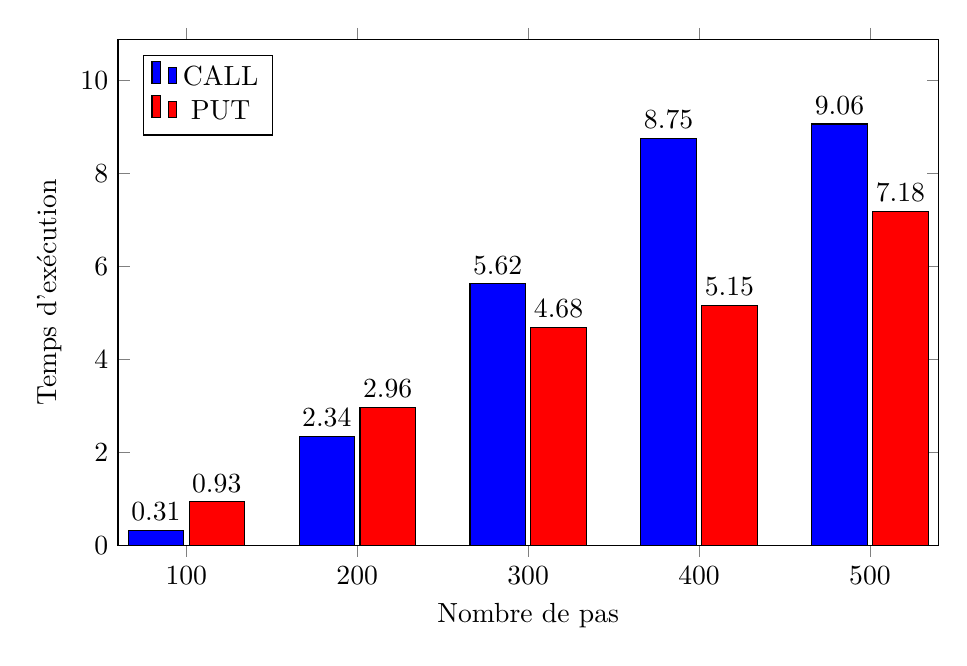
\begin{tikzpicture}caption{Evolution du temps d'exécution en fonction du type d'option}
    \begin{axis}[
        ybar,
        ymin=0,
        width  = 12cm,
        height = 8cm,
        bar width=20pt,
        ylabel={Temps d'exécution},
        xlabel={Nombre de pas},
        nodes near coords,
 %      nodes near coords align=below, % places labels inside bars
        symbolic x coords={100, 200, 300, 400, 500},
        xtick = data,
        enlarge y limits={value=0.2,upper},
        legend pos=north west
    ]
    \addplot[fill=blue] coordinates {(100, 0.31) (200, 2.34) (300, 5.62) (400, 8.75) (500, 9.06)};
     \addplot[fill=red] coordinates {(100, 0.93) (200, 2.96) (300, 4.68) (400, 5.15) (500, 7.18)};
   \legend{CALL,PUT}
\end{axis}
\end{tikzpicture} \\
%\caption{Evolution du temps d'exécution en fonction du type d'option}
%\label{participantsLanguageOverviewNonNative}
%\end{figure}
\begin{remark}
Le graphe ci-dessus représente l'évolution du temps d'exécution en fonction du type d'option.
Les temps d'exécution en ordonnées ont été multipliés par \textbf{10} afin d'avoir une meilleure visualisation.
\end{remark}

\begin{center}
        \textbf{Observations}
\end{center}
\begin{itemize}
\item Le temps d'exécution augmente avec le nombre de pas soit pour un call que pour un put.
\item Ensuite le temps d'exécution pour un call est plus important qu'un put quand le nombre de pas augmente. 
\item on constate une grande différence en terme de temps d'exécution quand on est entre 100 et 300 pas pour le call et le put, ensuite pour le call une différence moins importante entre les 400 et 500
 pas
 \end{itemize} 

%\begin{figure}
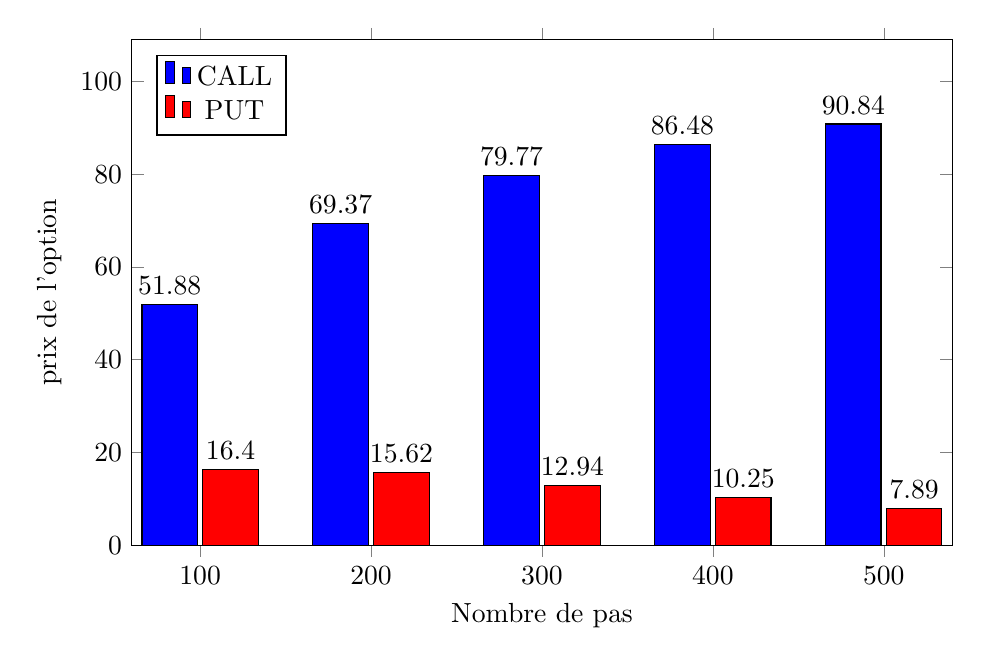
\begin{tikzpicture}caption{Evolution du temps d'exécution en fonction du type d'option}
    \begin{axis}[
        ybar,
        ymin=0,
        width  = 12cm,
        height = 8cm,
        bar width=20pt,
        ylabel={prix de l'option},
        xlabel={Nombre de pas},
        nodes near coords,
 %      nodes near coords align=below, % places labels inside bars
        symbolic x coords={100, 200, 300, 400, 500},
        xtick = data,
        enlarge y limits={value=0.2,upper},
        legend pos=north west
    ]
    \addplot[fill=blue] coordinates {(100, 51.88) (200, 69.37) (300, 79.77) (400, 86.48) (500, 90.84)};
     \addplot[fill=red] coordinates {(100, 16.40) (200, 15.62) (300, 12.94) (400, 10.25) (500, 7.89)};
   \legend{CALL,PUT}
\end{axis}
\end{tikzpicture} \\
%\caption{Evolution du temps d'exécution en fonction du type d'option}
%\label{participantsLanguageOverviewNonNative}
%\end{figure}
\begin{remark}
Le graphe suivant représente l'évolution du prix de l'option en fonction du type d'option

\end{remark}
\begin{center}
        \textbf{Observations}
\end{center}
\begin{itemize}
\item Le premier constant, est que le prix du call augmente en fonction de nombre de pas.
\item Le prix du put par-contre, diminue avec l'augmentation du nombre de pas.
\item Le constat majeur est le fait que le prix du call est trés supérieur à celui du put.
\end{itemize}

\begin{tabular}{|l|l|l|l|}
  \hline
  \multicolumn{4}{|c|}{Résultats  pour une \textbf{Option AMERICAINE} } \\
  \hline
  Type d'option & Nombre de pas & prix de l'option & Temps d'exécutuion(en secondes)\\ \hline
  \multirow{4}{*}{\textbf{CALL}} & 100 & 51.885144 & 0.169618 \\
    & 200 & 69.370564 & 1.04688 \\
    & 300 & 79.775962 & 1.0625 \\
    & 400 & 86.483306 & 1.32813 \\ 
    & 500 & 90.849835 & 1.64063 \\ \hline
  \multirow{4}{*}{\textbf{PUT}} & 100 & 20.300242 & 0.265625 \\
    & 200 & 24.198946 & 0.625 \\
    & 300 & 25.750120 & 1.1875 \\
    & 400 & 26.506822 & 1.89063 \\
    & 500 & 26.892057 & 1.90813 \\ \hline
\end{tabular} \\ \\

A partir de ce tableau, on vas essayer de créer des graphes afin d'avoir une interprétation plus efficace des résultats obtenus pour l'option AMERICAINE. \newline

%\begin{figure}
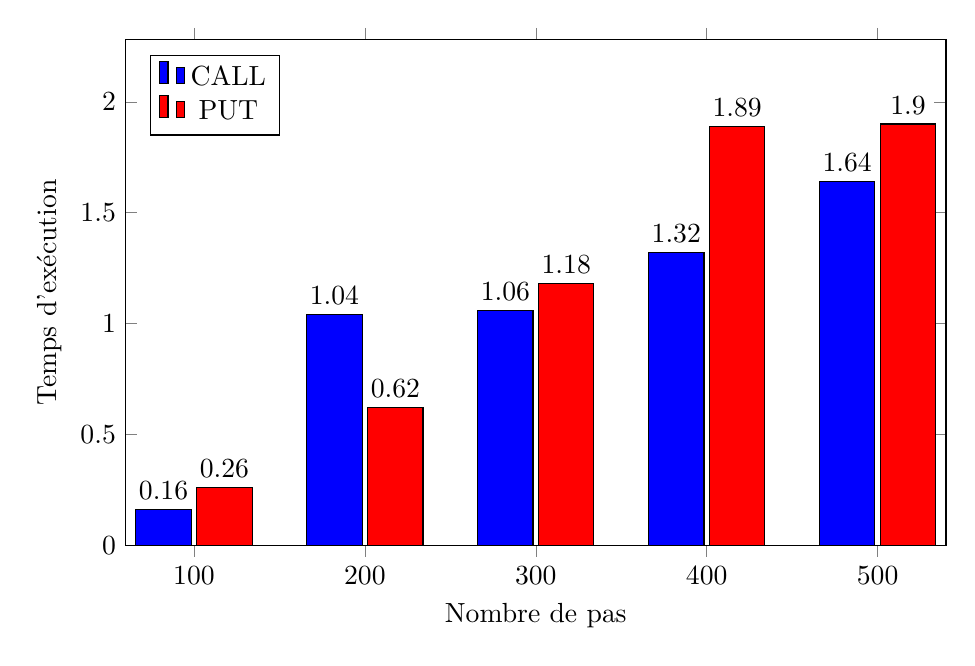
\begin{tikzpicture}caption{Evolution du temps d'exécution en fonction du type d'option}
    \begin{axis}[
        ybar,
        ymin=0,
        width  = 12cm,
        height = 8cm,
        bar width=20pt,
        ylabel={Temps d'exécution},
        xlabel={Nombre de pas},
        nodes near coords,
 %      nodes near coords align=below, % places labels inside bars
        symbolic x coords={100, 200, 300, 400, 500},
        xtick = data,
        enlarge y limits={value=0.2,upper},
        legend pos=north west
    ]
    \addplot[fill=blue] coordinates {(100, 0.16) (200, 1.04) (300, 1.06) (400, 1.32) (500, 1.64)};
     \addplot[fill=red] coordinates {(100, 0.26) (200, 0.62) (300, 1.18) (400, 1.89) (500, 1.90)};
   \legend{CALL,PUT}
\end{axis}
\end{tikzpicture} \\
%\caption{Evolution du temps d'exécution en fonction du type d'option}
%\label{participantsLanguageOverviewNonNative}
%\end{figure}
\begin{remark}
Le graphe ci-dessus représente l'évolution du temps d'exécution en fonction du type d'option.
\end{remark}

\begin{center}
        \textbf{Observations}
\end{center}
\begin{itemize}
\item Le temps d'exécution augmente avec le nombre de pas soit pour un call que pour un put.
\item Ensuite le temps d'exécution pour un call est plus important qu'un put quand le nombre de pas augmente. 
\item on constate une différence en terme de temps d'exécution quand on est entre 100 et 200 pas pour le call, ensuite pour le call et le put une différence moins importante entre les 300 et 500
 pas
 \end{itemize} 

%\begin{figure}
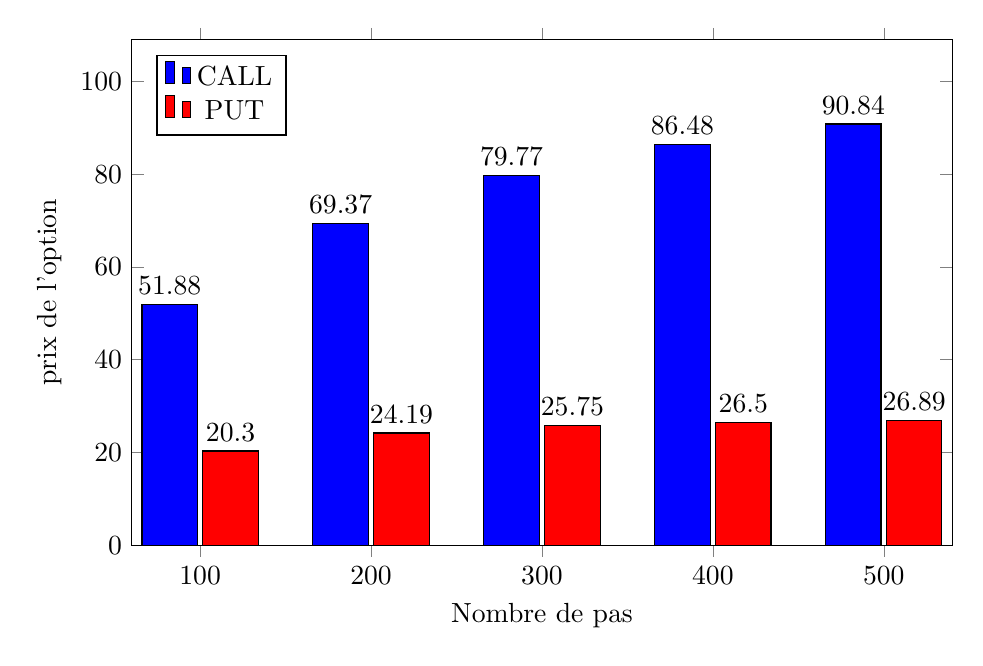
\begin{tikzpicture}caption{Evolution du temps d'exécution en fonction du type d'option}
    \begin{axis}[
        ybar,
        ymin=0,
        width  = 12cm,
        height = 8cm,
        bar width=20pt,
        ylabel={prix de l'option},
        xlabel={Nombre de pas},
        nodes near coords,
 %      nodes near coords align=below, % places labels inside bars
        symbolic x coords={100, 200, 300, 400, 500},
        xtick = data,
        enlarge y limits={value=0.2,upper},
        legend pos=north west
    ]
    \addplot[fill=blue] coordinates {(100, 51.88) (200, 69.37) (300, 79.77) (400, 86.48) (500, 90.84)};
     \addplot[fill=red] coordinates {(100, 20.30) (200, 24.19) (300, 25.75) (400, 26.50) (500, 26.89)};
   \legend{CALL,PUT}
\end{axis}
\end{tikzpicture} \\
%\caption{Evolution du temps d'exécution en fonction du type d'option}
%\label{participantsLanguageOverviewNonNative}
%\end{figure}
\begin{remark}
Le graphe suivant représente l'évolution du prix de l'option en fonction du type d'option
\end{remark}
\begin{center}
        \textbf{Observations}
\end{center}
\begin{itemize}
\item Le premier constant, est que le prix du call augmente en fonction de nombre de pas et on contaste que le prix est égale au prix du Call Europeen.
\item Le prix du put aussi augmente avec l'augmentation du nombre de pas comme contrairement au Put Europeen.
\item Le constat majeur est le fait que meme pour une option Americaine le prix du call est trés supérieur à celui du put.
\end{itemize}





%-------------------------------------------------------------------------
% Everything past here is required.  Do not delete these sections
% You can add to it if you wish.
%-------------------------------------------------------------------------
\newpage
\section{Partie 2 : CVAR}
Pour comprendre la CVaR, il est nécessaire d'avoir une défintion préliminaire de la VaR afin de comprendre d'où provient ce nouveau concept de CVaR.

\subsection{Définition VaR}
Les activités financières comportent des risques, même nos placements en actions présente 
un risque de perte de valeur en fonction des conditions du marché. Confrontés à ces risques, les institutions financières se sont munis au fil des années de techniques mathématiques sophistiquées.

Gérer ces risques nécessitent donc une bonne compréhension des mesures de risque quantitatives qui réfletent les vulnérabilités d'une entreprise, c'est ainsi que le ingénieurs financiers de \textbf{J.P. Morgan} ont développé la \textbf{VaR(Value at Risk)} qui est la mesure de risque la plus connue.

La \textbf{VaR(Value at Risk)} est une mesure liée au pourcentage de distributions de pertes et représente la perte maximale prévue avec un certain niveau de probabilité spécifié(ex: 95\%) sur une certaine période de temps(ex: un jour).

\begin{definition}{ \textbf{VaR}} \\
Considérons, par exemple, une variable aléatoire X qui représente la perte d'un portefeuille de placement sur une période de temps fixe. Une valeur négative pour X indique des gains. Étant donné un niveau de probabilité \texttt{$\alpha$},\texttt{$\alpha$}-VaR de la variable aléatoire X est donnée par la relation : 
\boldmath\begin{eqnarray}
VaR_{\alpha}(X) = \min{}(\gamma : P(X\ge1) \leq 1 - \alpha)
\end{eqnarray}
\end{definition}

%Lorsque la distribution des pertes est continue,VaR_{\alpha}(X) est simplement la perte telle que:
\boldmath\begin{eqnarray}
P(X\ge VaR_{\alpha}(X)) = \alpha
\end{eqnarray}


\subsection{Introduction de la CVaR}
Malgré cette popularité, la VaR a une importante propriété indésirable: elle manque de sous-ditivité.Une autre difficulté avec la VaR réside dans son calcul et son optimisation. Ces quelques caractéristiques indésirables de la VaR ont conduit à l'élaboration de mesures alternatives de risque, une des plus connues est la \textbf{CVaR(Conditional Value-at-Risk)}.\\
\begin{definition}{ \textbf{CVaR}} \\
Considérons un portefeuille d'actifs avec des rendements aléatoires. Désignons choix du portefeuille par le vecteur x et les événements aléatoires par le vecteur y. 
Soit f(x, y) la fonction de perte lorsque l'on choisit le portefeuille x d'un ensemble X des portefeuilles réalisables et y est la réalisation des événements aléatoires.Supposons que le vecteur aléatoire y a une fonction de densité de probabilité notée par p (y).
\boldmath\begin{eqnarray}
CVaR_{\alpha}(x) = \frac{1}{1-\alpha} \int_{f(x,y) \geq VaR_{\alpha}(x)}^{} f(x,y)p(y) dy
\end{eqnarray}
\end{definition}

\subsection{Minimisation CVaR}
La formule permettant de minimiser la CvaR est donnée par le programme linéaire suivant :
\begin{align}
\begin{split}
\text{min}\qquad &
   \gamma + \frac{1}{(1-\alpha)S} \sum_{s=1}^{S} z_{s} \\
  %&\qquad  +\sum_{\tau=t}^{t+T-1} [(X(\tau)+Y(\tau))(\gamma b(\tau)-\gamma v(\tau))]
  \end{split}
\label{green} 
\\[2ex]
\text{subject to}\qquad & z_{s} \geq 0, s = 1,...,S  %0\leq s(\tau)\leq s_{\textup{max}}, \quad \forall \tau   
\label{green-constraint-1} 
\\
& z_{s} \geq  f(x,y_{s}) - \gamma, s= 1,...,S  %\sum_{\tau=t}^{t+T-1} \gamma \beta(\tau)\leq N_{\textup{max}}
\label{green-constraint-2}
\\
& \sum_{i=1}^{n} \mu_{i}x_{i} \geq R
\label{green-constraint-3}
\\ & \sum_{i=1}^{n} x_{i} = 1
\label{green-constraint-4}
\\ &  x_{i} \geq 0
\end{align}

Il s'agit donc de résoudre un problème de programmation linéaire, en le résolvant on obtient le portefeuille x, l’espérance de rendement, la VaR et la CVaR. Par la suite nous analyserons sous forme de tableau les temps d'exécution en fonction des différentes instances.
\newline
\begin{center}
        \textbf{Analyse}
\end{center}

Pour résoudre ce programme nous considérerons les données suivantes:
\begin{itemize}
\item Scénarios: 1000, 3000, 5000
\item $\alpha$: 0.90
\item Nombre d'actifs: 100, 200, 300, 400, 500
\end{itemize}
Les autres variables du problème sont générées aléatoirement.\\ \\
\begin{tabular}{|l|l|l|l|l|}
  \hline
  \multicolumn{5}{|c|}{Résultat pour \textbf{$\alpha$ = 0.9} et \textbf{R = 10\%}} \\
  \hline
  Scénarios & Nombre d'actifs & VaR & CVaR & Temps d'exécutuion(en secondes)\\ \hline
  \multirow{5}{*}{1000} & 100 & 0.910021 & 0.960969 & 0.109375\\
    & 200 & 0.947418 & 1.000032 & 0.3125\\
    & 300 & 0.925309 & 0.975444 & 0.421875\\
    & 400 & 0.886986 & 0.948765 & 0.578125\\ 
    & 500 & 0.881355 & 0.940145 & 0.625\\ \hline
  \multirow{5}{*}{3000} & 100 & 0.887604 & 0.943919 & 1.01563\\
    & 200 & 0.897465 & 0.946905 & 1.6875\\
    & 300 & 0.911209 & 0.956905 & 2.45313\\
    & 400 & 0.929274 & 0.981281 & 2.875\\ 
    & 500 & 0.897495 & 0.950029 & 3.48438\\ \hline
  \multirow{5}{*}{5000} & 100 & 0.898341 & 0.949230 & 2.40625\\
    & 200 & 0.390625 & 0.949161 & 4.0625\\
    & 300 & 0.897875 & 0.948053 & 5.4375\\
    & 400 & 0.899941 & 0.950315 & 7.15625\\ 
    & 500 & 0.973881 & 1.027005 & 9.10938\\ \hline
\end{tabular} \\ \\

%\begin{figure}
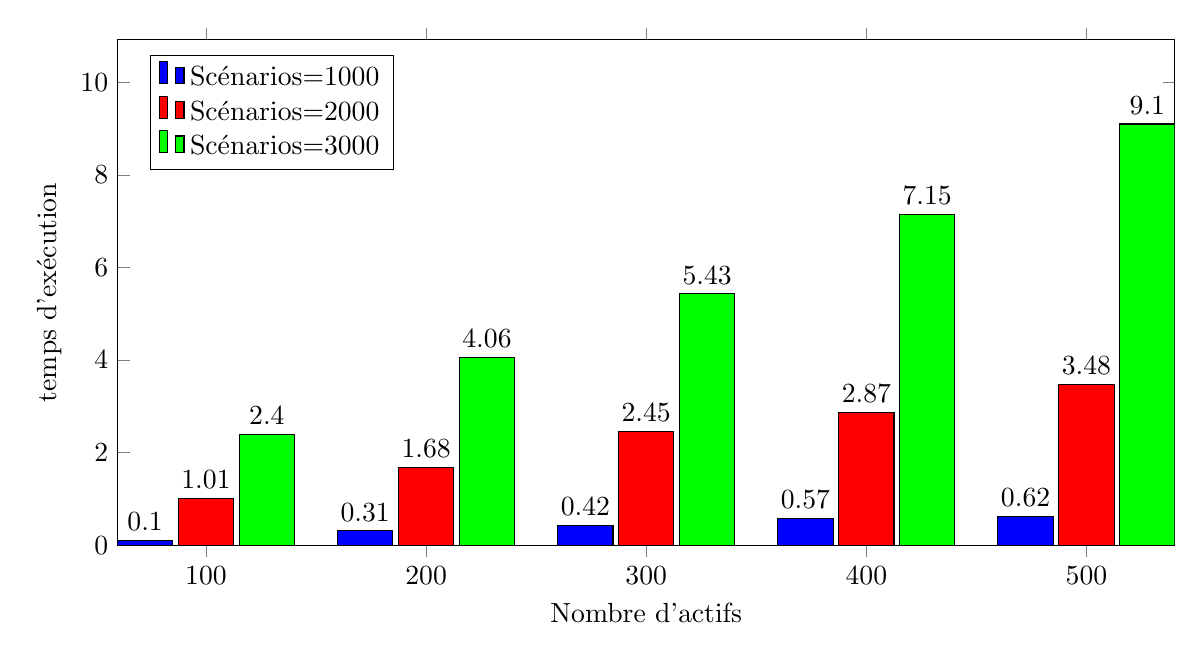
\begin{tikzpicture}
    \begin{axis}[
        ybar,
        ymin=0,
        width  = 15cm,
        height = 8cm,
        bar width=20pt,
        ylabel={temps d'exécution},
        xlabel={Nombre d'actifs},
        nodes near coords,
 %      nodes near coords align=below, % places labels inside bars
        symbolic x coords={100, 200, 300, 400, 500},
        xtick = data,
        enlarge y limits={value=0.2,upper},
        legend pos=north west
    ]
    \addplot[fill=blue] coordinates {(100, 0.10) (200, 0.31) (300, 0.42) (400, 0.57) (500, 0.62)};
     \addplot[fill=red] coordinates {(100, 1.01) (200, 1.68) (300, 2.45) (400, 2.87) (500, 3.48)};
     \addplot[fill=green] coordinates {(100, 2.40) (200, 4.06) (300, 5.43) (400, 7.15) (500, 9.10)};
   \legend{Scénarios=1000, Scénarios=2000, Scénarios=3000}
\end{axis}
\end{tikzpicture}
%\caption{Evolution du temps d'exécution en fonction du type d'option}
%\label{participantsLanguageOverviewNonNative}
%\end{figure}
\begin{remark}
Le graphe suivant représente l'évolution du temps d'exécution en fonction du nombre de scenarios et du nombre d'actifs avec un rendement attendu de \textbf{10\%}
\end{remark}

\begin{center}
        \textbf{Observations}
\end{center}
\begin{itemize}
\item On constate que les temps d'exécutions pour 1000 scénarios est la plus basse et celles pour 3000 scénarios est la plus haute
\item Pour chaque scénarios les temps d'exécutions augmentent en fonction du nombre d'actifs
\end{itemize}

%\begin{figure}
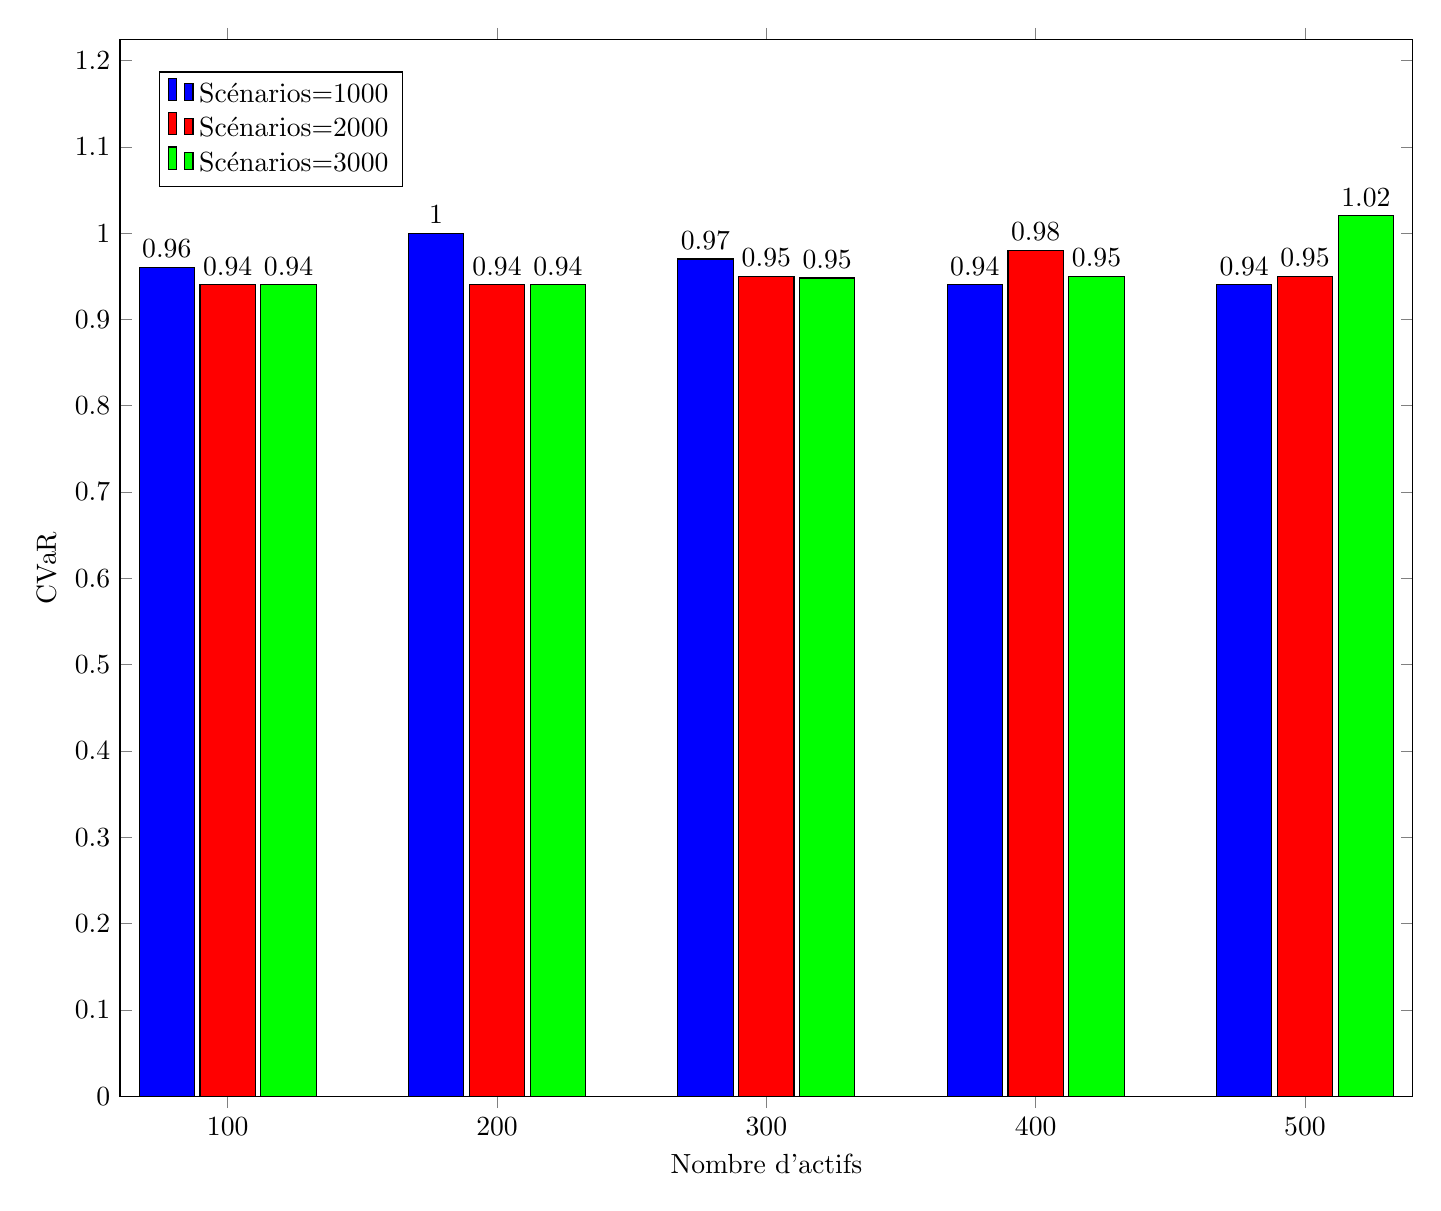
\begin{tikzpicture}
    \begin{axis}[
        ybar,
        ymin=0,
        width  = 18cm,
        height = 15cm,
        bar width=20pt,
        ylabel={CVaR},
        xlabel={Nombre d'actifs},
        nodes near coords,
 %      nodes near coords align=below, % places labels inside bars
        symbolic x coords={100, 200, 300, 400, 500},
        xtick = data,
        enlarge y limits={value=0.2,upper},
        legend pos=north west
    ]
    \addplot[fill=blue] coordinates {(100, 0.96) (200, 1.00) (300, 0.97) (400, 0.94) (500, 0.94)};
     \addplot[fill=red] coordinates {(100, 0.94) (200, 0.94) (300, 0.95) (400, 0.98) (500, 0.95)};
     \addplot[fill=green] coordinates {(100, 0.94) (200, 0.94) (300, 0.948) (400, 0.95) (500, 1.02)};
   \legend{Scénarios=1000, Scénarios=2000, Scénarios=3000}
\end{axis}
\end{tikzpicture}
%\caption{Evolution du temps d'exécution en fonction du type d'option}
%\label{participantsLanguageOverviewNonNative}
%\end{figure}
\begin{remark}
Le graphe suivant représente l'évolution de la CVaR en fonction du nombre de scenarios et du nombre d'actifs avec un rendement attendu de \textbf{10\%}
\end{remark}

\begin{center}
        \textbf{Observations}
\end{center}
\begin{itemize}
\item On observe que globalment la valeur de la CVaR oscille entre 0.9 et 1 pour chaque scénarios.
\item Et d'aprés le tableau on observe que la CVaR est au dessus de la VaR.
\end{itemize}

\begin{tabular}{|l|l|l|l|l|}
  \hline
  \multicolumn{5}{|c|}{Résultat pour \textbf{$\alpha$ = 0.90} et \textbf{R = 20\%}} \\
  \hline
  Scénarios & Nombre d'actifs & VaR & CVaR & Temps d'exécutuion(en secondes)\\ \hline
  \multirow{5}{*}{1000} & 100 & 0.886233 & 0.945663 & 0.171875\\
    & 200 & 0.904963 & 0.956746 & 0.265625\\
    & 300 & 0.926559 & 0.968807 & 0.46875\\
    & 400 & 1.05394 & 1.123643 & 0.65625\\ 
    & 500 & 0.907796 & 0.953035 & 0.75\\ \hline
  \multirow{5}{*}{3000} & 100 & 0.901170 & 0.950043 & 1.14063\\
    & 200 & 0.959994 & 1.008004 & 1.78125\\
    & 300 & 0.904301 & 0.950364 & 2.32813\\
    & 400 & 0.891909 & 0.943455 & 3.20313\\ 
    & 500 & 0.899648 & 0.947596 & 3.75\\ \hline
  \multirow{5}{*}{5000} & 100 & 0.901068 & 0.949867 & 2.75\\
    & 200 & 0.894601 & 0.946562 & 4.32813\\
    & 300 & 0.908569 & 0.953732 & 6.57813\\
    & 400 & 0.903140 & 0.953964 & 8.15625\\ 
    & 500 & 0.895939 & 0.949594 & 9.23438\\ \hline
  %\multirow{2}{*}{Attaquants} & ST & Alan Smith \\
   % & ST & Mark Viduka \\
 %\hline
\end{tabular}

%\begin{figure}
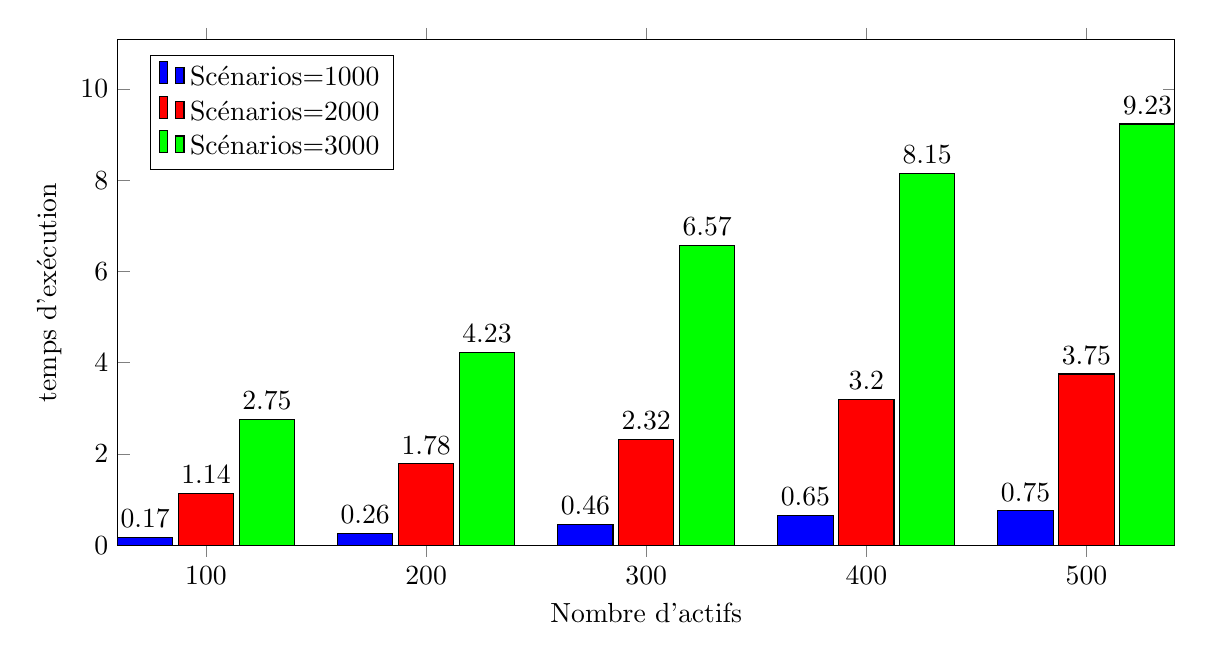
\begin{tikzpicture}
    \begin{axis}[
        ybar,
        ymin=0,
        width  = 15cm,
        height = 8cm,
        bar width=20pt,
        ylabel={temps d'exécution},
        xlabel={Nombre d'actifs},
        nodes near coords,
 %      nodes near coords align=below, % places labels inside bars
        symbolic x coords={100, 200, 300, 400, 500},
        xtick = data,
        enlarge y limits={value=0.2,upper},
        legend pos=north west
    ]
    \addplot[fill=blue] coordinates {(100, 0.17) (200, 0.26) (300, 0.46) (400, 0.65) (500, 0.75)};
     \addplot[fill=red] coordinates {(100, 1.14) (200, 1.78) (300, 2.32) (400, 3.20) (500, 3.75)};
     \addplot[fill=green] coordinates {(100, 2.75) (200, 4.23) (300, 6.57) (400, 8.15) (500, 9.23)};
   \legend{Scénarios=1000, Scénarios=2000, Scénarios=3000}
\end{axis}
\end{tikzpicture}
%\caption{Evolution du temps d'exécution en fonction du type d'option}
%\label{participantsLanguageOverviewNonNative}
%\end{figure}
\begin{remark}
Le graphe suivant représente l'évolution du temps d'exécution en fonction du nombre de scenarios et du nombre d'actifs avec un rendement attendu de \textbf{20\%}
\end{remark}

\begin{center}
        \textbf{Observations}
\end{center}
\begin{itemize}
\item On constate que les temps d'exécutions pour 1000 scénarios est la plus basse et celles pour 3000 scénarios est la plus haute malgré l'augmentation du rendement attendu.
\item Pour chaque scénarios les temps d'exécutions augmentent en fonction du nombre d'actifs, on constate aussi que le temps d'exécution est légérement supérieur par rapport au graphe précédent 
\end{itemize}

%\begin{figure}
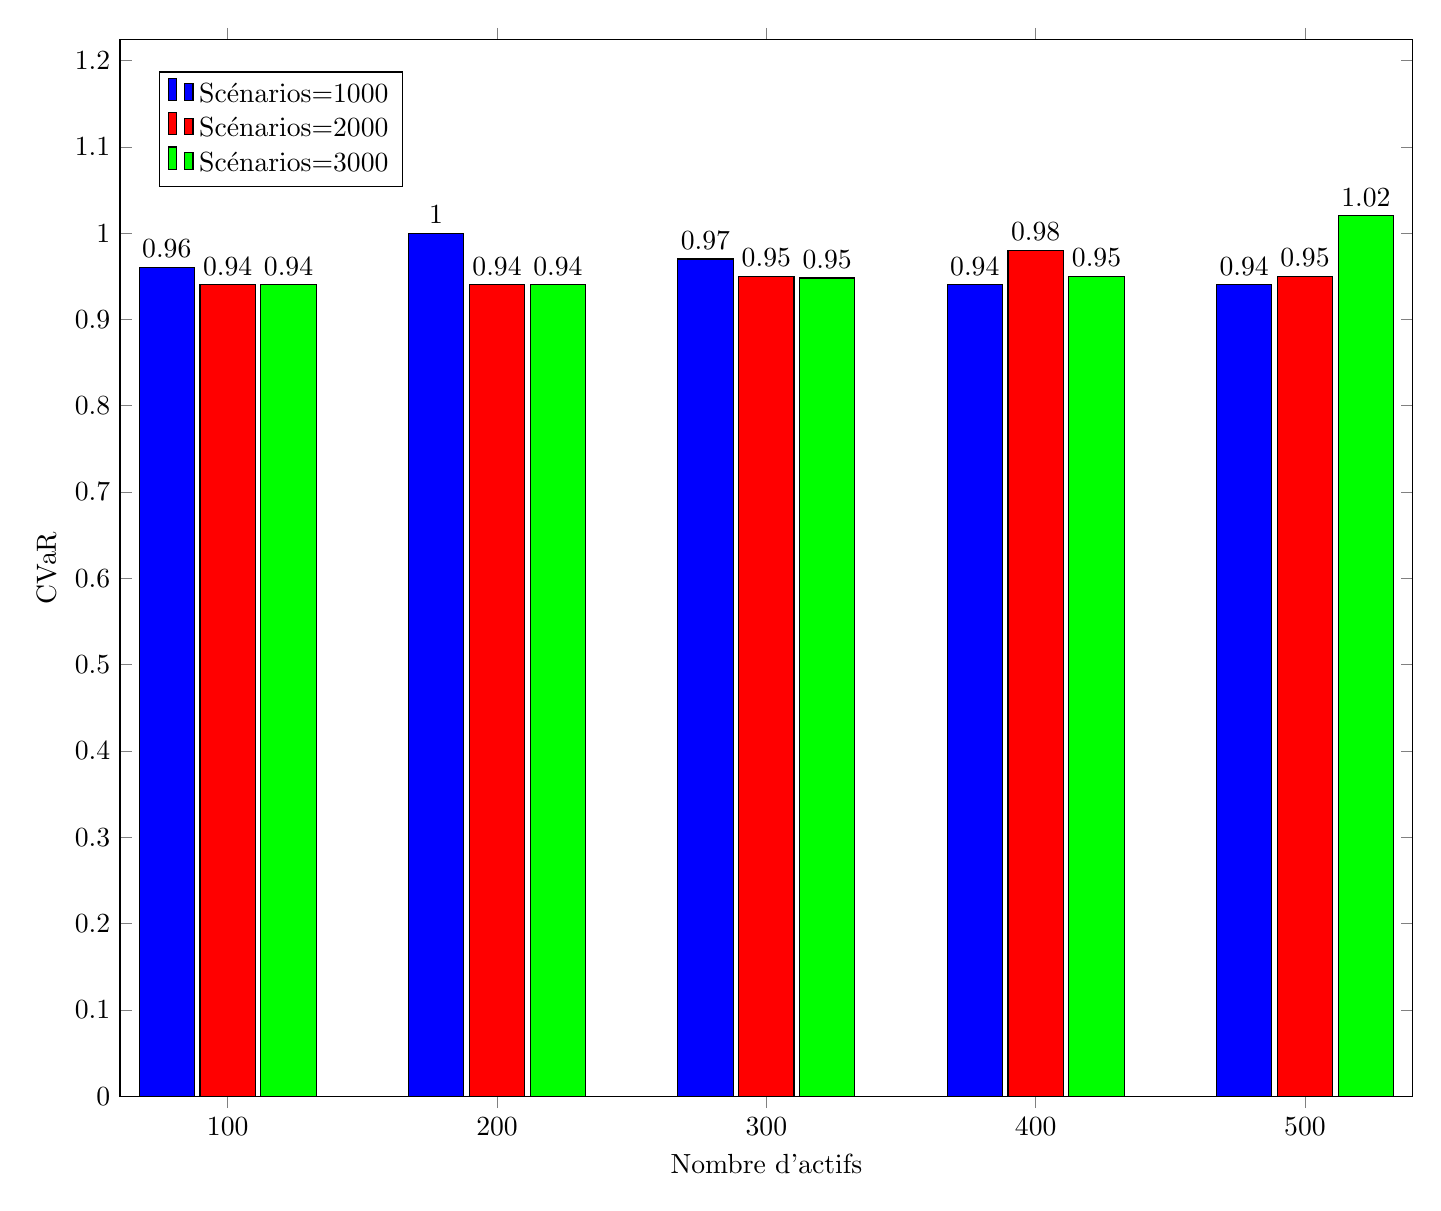
\begin{tikzpicture}
    \begin{axis}[
        ybar,
        ymin=0,
        width  = 18cm,
        height = 15cm,
        bar width=20pt,
        ylabel={CVaR},
        xlabel={Nombre d'actifs},
        nodes near coords,
 %      nodes near coords align=below, % places labels inside bars
        symbolic x coords={100, 200, 300, 400, 500},
        xtick = data,
        enlarge y limits={value=0.2,upper},
        legend pos=north west
    ]
    \addplot[fill=blue] coordinates {(100, 0.96) (200, 1.00) (300, 0.97) (400, 0.94) (500, 0.94)};
     \addplot[fill=red] coordinates {(100, 0.94) (200, 0.94) (300, 0.95) (400, 0.98) (500, 0.95)};
     \addplot[fill=green] coordinates {(100, 0.94) (200, 0.94) (300, 0.948) (400, 0.95) (500, 1.02)};
   \legend{Scénarios=1000, Scénarios=2000, Scénarios=3000}
\end{axis}
\end{tikzpicture}
%\caption{Evolution du temps d'exécution en fonction du type d'option}
%\label{participantsLanguageOverviewNonNative}
%\end{figure}
\begin{remark}
Le graphe suivant représente l'évolution de la CVaR en fonction du nombre de scenarios et du nombre d'actifs avec un rendement attendu de \textbf{20\%}
\end{remark}

\begin{center}
        \textbf{Observations}
\end{center}
\begin{itemize}
\item On observe que globalement la valeur de la CVaR oscille entre 0.9 et 1 pour chaque scénarios malgré l'augmentation du rendement, la fait que notre CVaR oscille entre ces valeurs est surement du au caractére aléatoire de nos données, que nous avons choisis trés petites.
\item De meme la CVaR reste toujours au dessus de la VaR, ce qui nous permet de d'affirmer que notre modélisation est correcte.
\end{itemize}



\subsection{Maximisation CVaR}
La formule permettant de maximiser la CvaR est donnée par le programme linéaire suivant :
\begin{align}
\begin{split}
\text{max}\qquad & \sum_{i=1}^{n} \mu_{i}x_{i} 
  \end{split}
\label{green} 
\\[2ex]
\text{subject to}\qquad &  \gamma + \frac{1}{(1-\alpha_{j})S} \sum_{s=1}^{S} z_{s} \leq U_{\alpha_{j}} , j = 1,...,J
\label{green-constraint-1} 
\\
& z_{s} \geq 0 s = 1,...,S 
\label{green-constraint-1} 
\\
& z_{s} \geq  f(x,y_{s}) - \gamma  
\label{green-constraint-2}
\\ & \sum_{i=1}^{n} x_{i} = 1
\label{green-constraint-4}
\\ & l_{i}\leq x_{i} \leq u_{i}, i = 1,...,n
\label{green-constraint-4}
\\ &  x_{i} \geq 0
\end{align}

Comme précédement, il s'agit d'un problème de programmation linéaire, et nous ferons les analyses avec les meme données.
\newline
\begin{center}
        \textbf{Analyse}
\end{center}

Pour résoudre ce programme nous considérerons les données suivantes:
\begin{itemize}
\item Scénarios: 1000, 3000, 5000
\item $\alpha$: 0.90, 0.96
\item Nombre d'actifs: 100, 200, 300, 400, 500
\end{itemize}
Les autres variables du problème sont générées aléatoirement.\\ \\
\begin{tabular}{|l|l|l|l|l|}
  \hline
  \multicolumn{5}{|c|}{Résultat pour \textbf{$\alpha$ = 0.9} et \textbf{R = 10\%}} \\
  \hline
  Scénarios & Nombre d'actifs & VaR & CVaR & Temps d'exécutuion(en secondes)\\ \hline
  \multirow{5}{*}{1000} & 100 & 0.910021 & 0.960969 & 0.209375\\
    & 200 & 0.947418 & 1.000032 & 0.4125\\
    & 300 & 0.925309 & 0.975444 & 0.621875\\
    & 400 & 0.886986 & 0.948765 & 0.978125\\ 
    & 500 & 0.881355 & 0.940145 & 1.625\\ \hline
  \multirow{5}{*}{3000} & 100 & 0.887604 & 0.943919 & 1.71563\\
    & 200 & 0.897465 & 0.946905 & 2.6875\\
    & 300 & 0.911209 & 0.946905 & 3.5313\\
    & 400 & 0.929274 & 0.981281 & 3.75\\ 
    & 500 & 0.897495 & 0.950029 & 4.8438\\ \hline
  \multirow{5}{*}{5000} & 100 & 0.898341 & 0.949230 & 2.78625\\
    & 200 & 0.390625 & 0.949161 & 4.2625\\
    & 300 & 0.897875 & 0.948053 & 6.5875\\
    & 400 & 0.899941 & 0.950315 & 8.15625\\ 
    & 500 & 0.973881 & 1.027005 & 9.23938\\ \hline
\end{tabular} \\ \\
%\begin{figure}
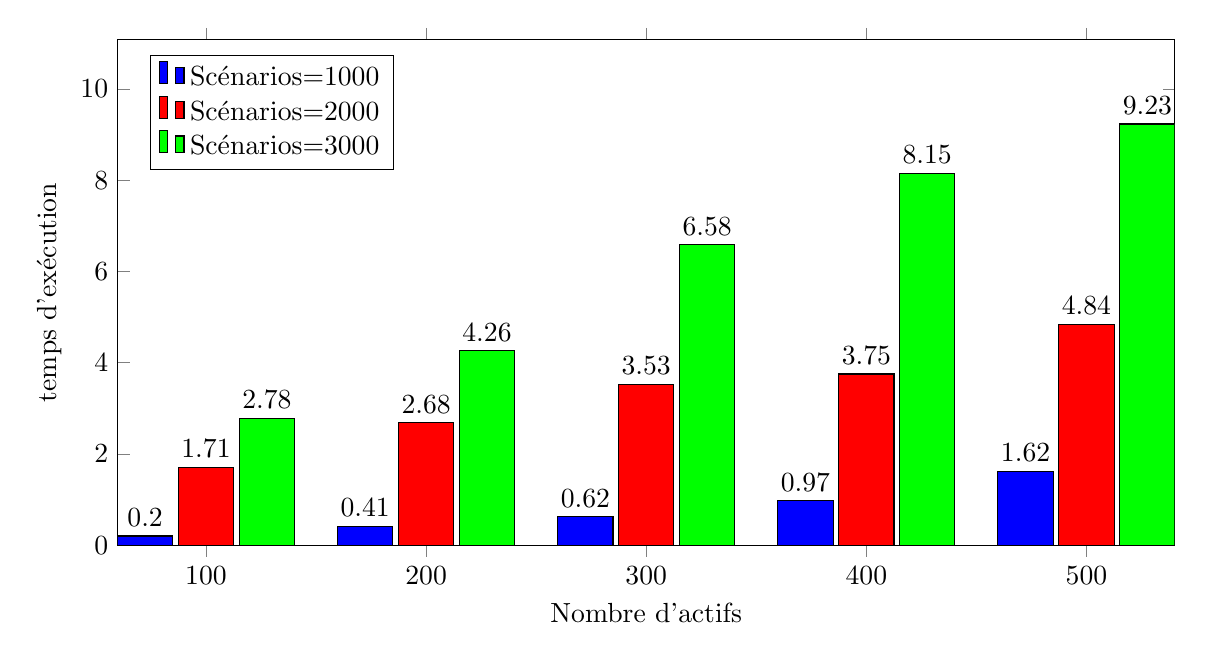
\begin{tikzpicture}
    \begin{axis}[
        ybar,
        ymin=0,
        width  = 15cm,
        height = 8cm,
        bar width=20pt,
        ylabel={temps d'exécution},
        xlabel={Nombre d'actifs},
        nodes near coords,
 %      nodes near coords align=below, % places labels inside bars
        symbolic x coords={100, 200, 300, 400, 500},
        xtick = data,
        enlarge y limits={value=0.2,upper},
        legend pos=north west
    ]
    \addplot[fill=blue] coordinates {(100, 0.20) (200, 0.41) (300, 0.62) (400, 0.97) (500, 1.62)};
     \addplot[fill=red] coordinates {(100, 1.71) (200, 2.68) (300, 3.53) (400, 3.75) (500, 4.84)};
     \addplot[fill=green] coordinates {(100, 2.78) (200, 4.26) (300, 6.58) (400, 8.15) (500, 9.23)};
   \legend{Scénarios=1000, Scénarios=2000, Scénarios=3000}
\end{axis}
\end{tikzpicture}
%\caption{Evolution du temps d'exécution en fonction du type d'option}
%\label{participantsLanguageOverviewNonNative}
%\end{figure}
\begin{remark}
Le graphe suivant représente l'évolution du temps d'exécution en fonction du nombre de scenarios et du nombre d'actifs avec un rendement attendu de \textbf{10\%}
\end{remark}

\begin{center}
        \textbf{Observations}
\end{center}
\begin{itemize}
\item On constate que les temps d'exécutions pour 1000 scénarios est la plus basse et celles pour 3000 scénarios est la plus haute malgré l'augmentation du rendement attendu.
\item Pour chaque scénarios les temps d'exécutions augmentent en fonction du nombre d'actifs
\end{itemize}

%\begin{figure}
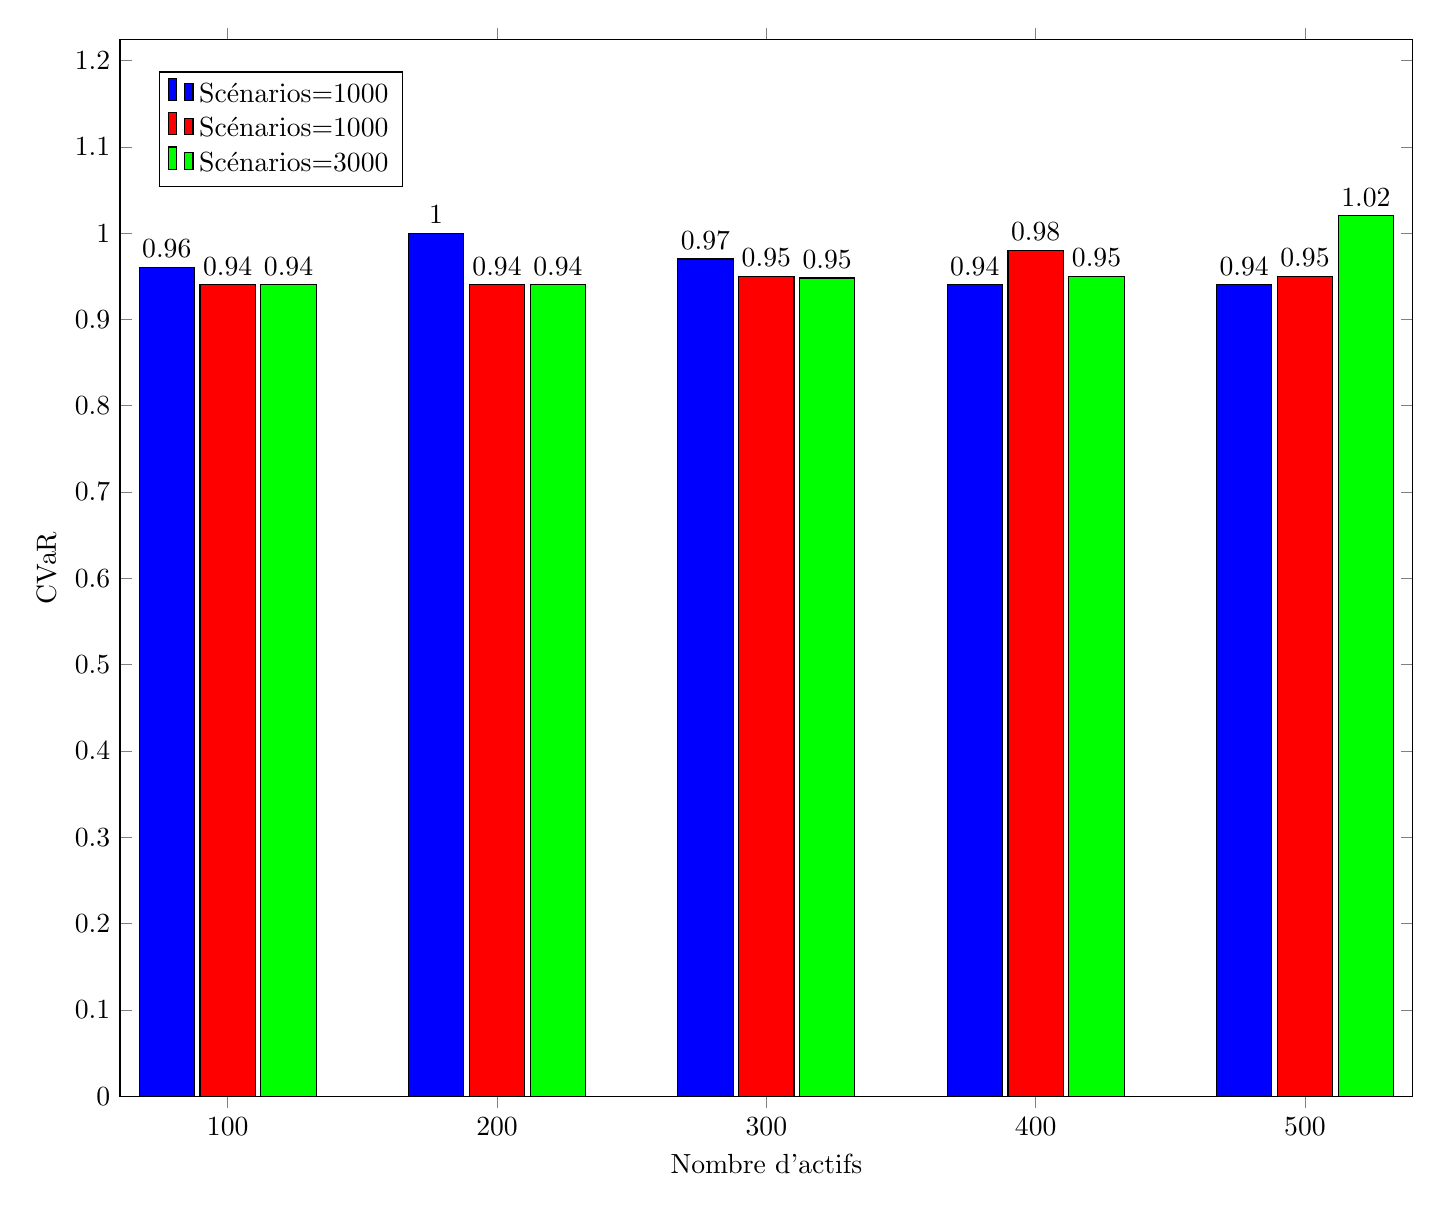
\begin{tikzpicture}
    \begin{axis}[
        ybar,
        ymin=0,
        width  = 18cm,
        height = 15cm,
        bar width=20pt,
        ylabel={CVaR},
        xlabel={Nombre d'actifs},
        nodes near coords,
 %      nodes near coords align=below, % places labels inside bars
        symbolic x coords={100, 200, 300, 400, 500},
        xtick = data,
        enlarge y limits={value=0.2,upper},
        legend pos=north west
    ]
    \addplot[fill=blue] coordinates {(100, 0.96) (200, 1.00) (300, 0.97) (400, 0.94) (500, 0.94)};
     \addplot[fill=red] coordinates {(100, 0.94) (200, 0.94) (300, 0.95) (400, 0.98) (500, 0.95)};
     \addplot[fill=green] coordinates {(100, 0.94) (200, 0.94) (300, 0.948) (400, 0.95) (500, 1.02)};
   \legend{Scénarios=1000, Scénarios=1000, Scénarios=3000}
\end{axis}
\end{tikzpicture}
%\caption{Evolution du temps d'exécution en fonction du type d'option}
%\label{participantsLanguageOverviewNonNative}
%\end{figure}
\begin{remark}
Le graphe suivant représente l'évolution du temps d'exécution en fonction du nombre de scenarios et du nombre d'actifs avec un rendement attendu de \textbf{10\%}
\end{remark}

\begin{center}
        \textbf{Observations}
\end{center}
\begin{itemize}
\item On observe que globalement la valeur de la CVaR oscille entre 0.9 et 1 pour chaque scénarios malgré l'augmentation du rendement.
\end{itemize}
\begin{tabular}{|l|l|l|l|l|}
  \hline
  \multicolumn{5}{|c|}{Résultat pour \textbf{$\alpha$ = 0.90} et \textbf{R = 20\%}} \\
  \hline
  Scénarios & Nombre d'actifs & VaR & CVaR & Temps d'exécutuion(en secondes)\\ \hline
  \multirow{5}{*}{1000} & 100 & 0.886233 & 0.945663 & 0.171875\\
    & 200 & 0.904963 & 0.956746 & 0.265625\\
    & 300 & 0.926559 & 0.968807 & 0.46875\\
    & 400 & 1.05394 & 1.123643 & 0.65625\\ 
    & 500 & 0.907796 & 0.953035 & 0.75\\ \hline
  \multirow{5}{*}{3000} & 100 & 0.901170 & 0.950043 & 1.14063\\
    & 200 & 0.959994 & 1.008004 & 1.78125\\
    & 300 & 0.904301 & 0.950364 & 2.32813\\
    & 400 & 0.891909 & 0.943455 & 3.20313\\ 
    & 500 & 0.899648 & 0.947596 & 3.75\\ \hline
  \multirow{5}{*}{5000} & 100 & 0.901068 & 0.949867 & 2.75\\
    & 200 & 0.894601 & 0.946562 & 4.89813\\
    & 300 & 0.908569 & 0.953732 & 7.57813\\
    & 400 & 0.903140 & 0.953964 & 8.45625\\ 
    & 500 & 0.895939 & 0.949594 & 10.50438\\ \hline
  %\multirow{2}{*}{Attaquants} & ST & Alan Smith \\
   % & ST & Mark Viduka \\
 %\hline
\end{tabular}

%\begin{figure}
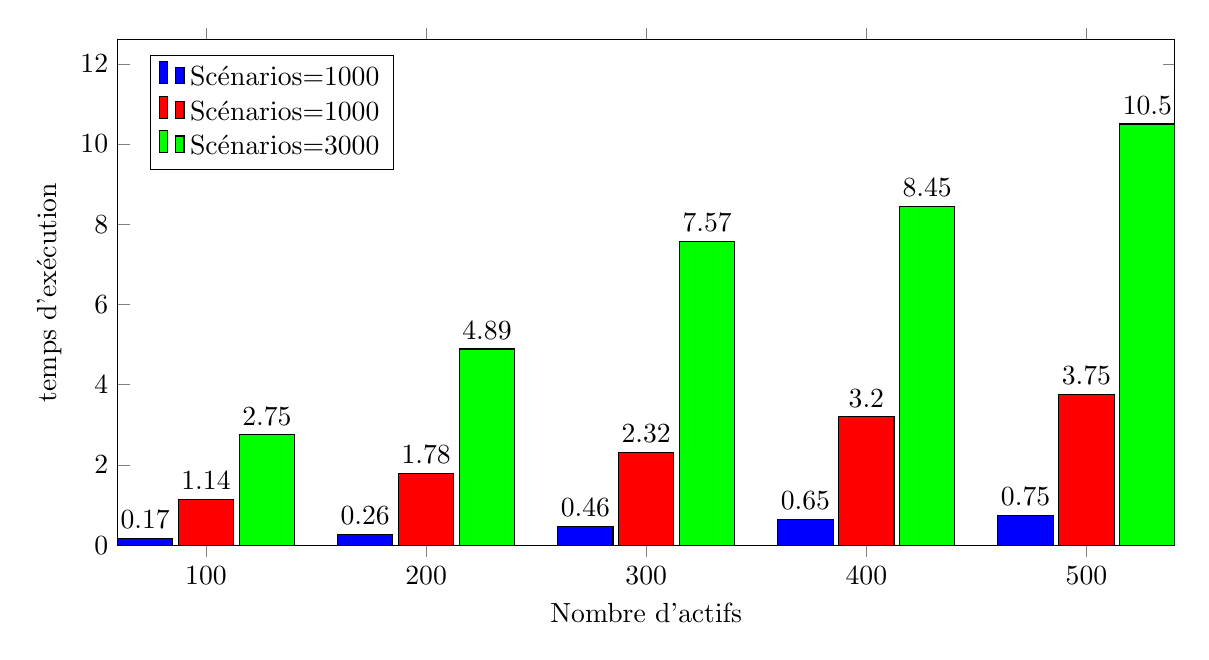
\begin{tikzpicture}
    \begin{axis}[
        ybar,
        ymin=0,
        width  = 15cm,
        height = 8cm,
        bar width=20pt,
        ylabel={temps d'exécution},
        xlabel={Nombre d'actifs},
        nodes near coords,
 %      nodes near coords align=below, % places labels inside bars
        symbolic x coords={100, 200, 300, 400, 500},
        xtick = data,
        enlarge y limits={value=0.2,upper},
        legend pos=north west
    ]
    \addplot[fill=blue] coordinates {(100, 0.17) (200, 0.26) (300, 0.46) (400, 0.65) (500, 0.75)};
     \addplot[fill=red] coordinates {(100, 1.14) (200, 1.78) (300, 2.32) (400, 3.20) (500, 3.75)};
     \addplot[fill=green] coordinates {(100, 2.75) (200, 4.89) (300, 7.57) (400, 8.45) (500, 10.50)};
   \legend{Scénarios=1000, Scénarios=1000, Scénarios=3000}
\end{axis}
\end{tikzpicture}
%\caption{Evolution du temps d'exécution en fonction du type d'option}
%\label{participantsLanguageOverviewNonNative}
%\end{figure}
\begin{remark}
Le graphe suivant représente l'évolution du temps d'exécution en fonction du nombre de scenarios et du nombre d'actifs avec un rendement attendu de \textbf{20\%}
\end{remark}

\begin{center}
        \textbf{Observations}
\end{center}
\begin{itemize}
\item On constate que les temps d'exécutions pour 1000 scénarios est la plus basse et celles pour 3000 scénarios est la plus haute malgré l'augmentation du rendement attendu.
\item Pour chaque scénarios les temps d'exécutions augmentent en fonction du nombre d'actifs
\end{itemize}

%\begin{figure}
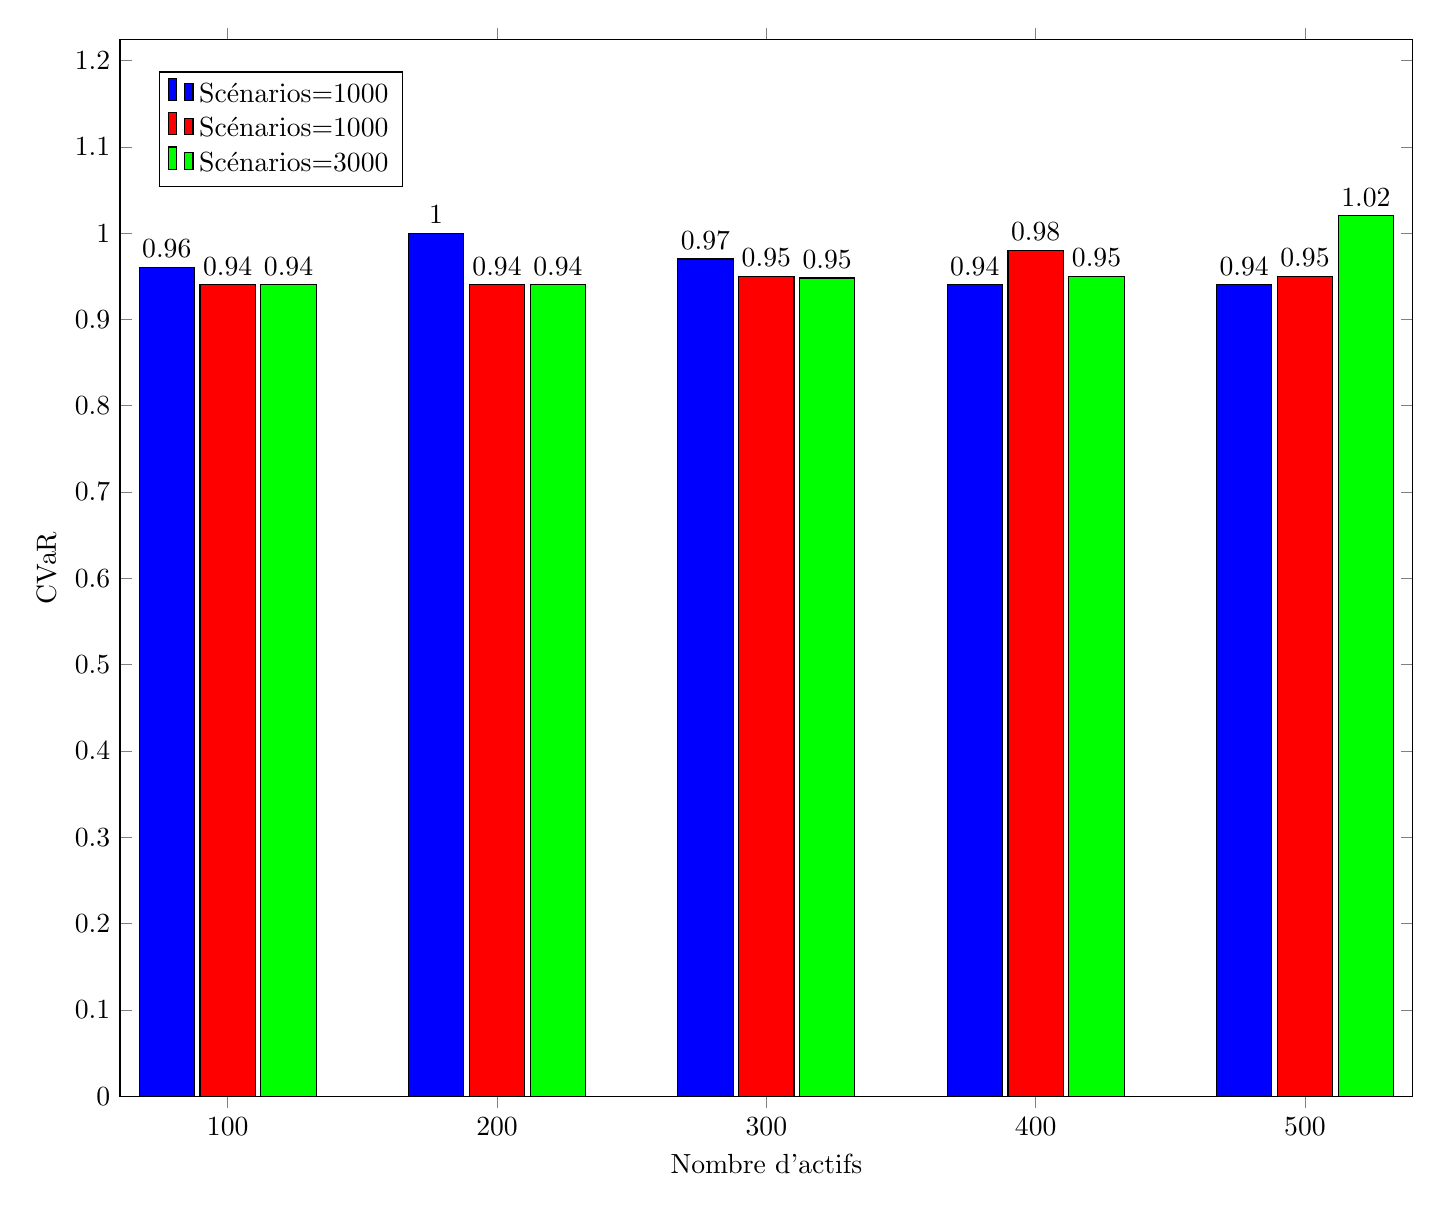
\begin{tikzpicture}
    \begin{axis}[
        ybar,
        ymin=0,
        width  = 18cm,
        height = 15cm,
        bar width=20pt,
        ylabel={CVaR},
        xlabel={Nombre d'actifs},
        nodes near coords,
 %      nodes near coords align=below, % places labels inside bars
        symbolic x coords={100, 200, 300, 400, 500},
        xtick = data,
        enlarge y limits={value=0.2,upper},
        legend pos=north west
    ]
    \addplot[fill=blue] coordinates {(100, 0.96) (200, 1.00) (300, 0.97) (400, 0.94) (500, 0.94)};
     \addplot[fill=red] coordinates {(100, 0.94) (200, 0.94) (300, 0.95) (400, 0.98) (500, 0.95)};
     \addplot[fill=green] coordinates {(100, 0.94) (200, 0.94) (300, 0.948) (400, 0.95) (500, 1.02)};
   \legend{Scénarios=1000, Scénarios=1000, Scénarios=3000}
\end{axis}
\end{tikzpicture}
%\caption{Evolution du temps d'exécution en fonction du type d'option}
%\label{participantsLanguageOverviewNonNative}
%\end{figure}
\begin{remark}
Le graphe suivant représente l'évolution du temps d'exécution en fonction du nombre de scenarios et du nombre d'actifs avec un rendement attendu de \textbf{20\%}
\end{remark}

\begin{center}
        \textbf{Observations}
\end{center}
\begin{itemize}
\item On observe que globalement la valeur de la CVaR oscille entre 0.9 et 1 pour chaque scénarios malgré l'augmentation du rendement.
\end{itemize}

 \newpage
 \appendix
 \section{Appendix 1}
% This is a very short example of doing an appendix in \LaTeX.  An appendix is not required but is a good place to put code, additional drawings, tables or other information that will help the instructor in determining that you met the requirements of the milestone.  I have included an example of how you can use \LaTeX to automatically import code.

% % The following tells listings how to treat the code.  You can edit this
% % as needed

% \lstset{language=Matlab,%
%     %basicstyle=\color{red},
%     breaklines=true,%
%     morekeywords={matlab2tikz},
%     keywordstyle=\color{blue},%
%     morekeywords=[2]{1}, keywordstyle=[2]{\color{black}},
%     identifierstyle=\color{black},%
%     stringstyle=\color{mylilas},
%     commentstyle=\color{mygreen},%
%     showstringspaces=false,%without this there will be a symbol in the places where there is a space
%     numbers=left,%
%     numberstyle={\tiny \color{black}},% size of the numbers
%     numbersep=9pt, % this defines how far the numbers are from the text
%     emph=[1]{for,end,break},emphstyle=[1]\color{red}, %some words to emphasise
%     %emph=[2]{word1,word2}, emphstyle=[2]{style},    
% }

% % To import your code, just use the following command.  Make sure it is the same
% % folder or if using Overleaf it is uploaded to the project.
\let\ph\mlplaceholder % shorter macro
\lstMakeShortInline"

\lstset{
  style              = Matlab-editor,
  basicstyle         = \mlttfamily,
  escapechar         = ",
  mlshowsectionrules = true,
}
 \lstinputlisting[caption = {exercise type class definition}]{ExerciseType.m}
 
 \lstinputlisting[caption = {option type class definition}]{OptionType.m}
 
 \lstinputlisting[caption = {pricing main class definition}]{binomial_tree_pricing.m}


% %-------------------------------------------------------------------------
% % DO NOT DELETE THIS.
% % This is the end of the document.  Nothing else should go past this.
% %-------------------------------------------------------------------------

\section{Appendix 2}

\lstinputlisting[caption = {CvaR minimisation class definition}]{cvar_min.m}
\newpage
\lstinputlisting[caption = {CvaR maximisation class definition}]{cvar_max.m}

\end{document}